\documentclass[border=6pt]{standalone}
\usepackage{fontspec}
\defaultfontfeatures{Ligatures=TeX}
\setmainfont{Palatino Linotype}
\usepackage{tikz}
\usetikzlibrary{arrows.meta, positioning, calc, shapes.geometric, fit,
                backgrounds, decorations.pathmorphing}
\definecolor{casink}{HTML}{1A1A22}
\definecolor{casaccent}{HTML}{6B3F8C}
\definecolor{casmuted}{HTML}{8A8A94}
\definecolor{caswash}{HTML}{F0ECF4}

\tikzset{
  casnode/.style={
    draw=casink, line width=0.5pt, rounded corners=1.2pt,
    fill=caswash, inner sep=3.2pt, font=\small, minimum height=6.5mm,
    align=center},
  casdomain/.style={
    casnode, minimum width=34mm, font=\small\bfseries},
  casflow/.style={
    -{Stealth[length=2.1mm,width=1.6mm]}, draw=casink, line width=0.55pt},
  casfeedback/.style={
    -{Stealth[length=2.1mm,width=1.6mm]}, draw=casmuted, line width=0.5pt,
    dashed, dash pattern=on 1.6pt off 1.4pt},
  casinvol/.style={
    {Stealth[length=1.8mm,width=1.4mm]}-{Stealth[length=1.8mm,width=1.4mm]},
    draw=casaccent, line width=0.5pt},
  caslabel/.style={font=\scriptsize, text=casmuted},
  cascap/.style={font=\scriptsize\itshape, text=casink},
}

% Every figure in this book uses the same wrapper so the list of figures and
% the numbering stay consistent.
\newcommand{\casfig}[3]{%
  \begin{figure}[htbp]
  \centering
  #2
  \caption{#3}\label{fig:#1}
  \end{figure}%
}

\begin{document}

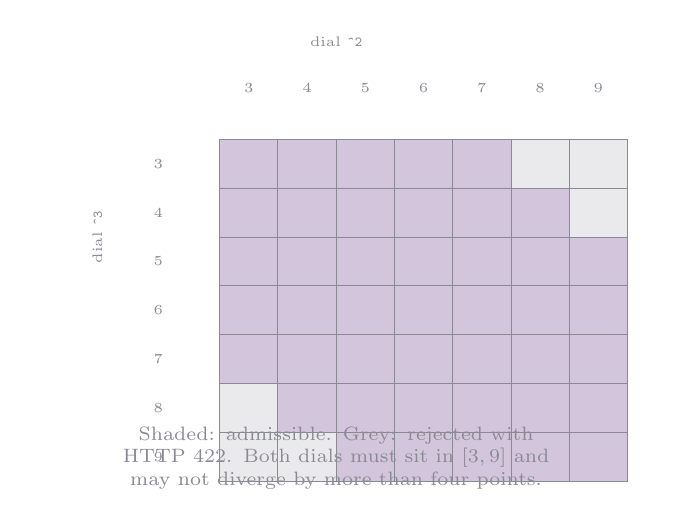
\begin{tikzpicture}[x=7.4mm, y=6.2mm]
  % Legal band for an involution pair: |a - b| <= 4, each in [3,9].
  \foreach \v in {3,4,5,6,7,8,9} {
    \node[caslabel, font=\tiny] at (\v-2, 0.55) {\v};
    \node[caslabel, font=\tiny] at (-0.55, -\v+2) {\v};
  }
  \foreach \a in {3,...,9} {
    \foreach \b in {3,...,9} {
      \pgfmathtruncatemacro\diff{abs(\a-\b)}
      \ifnum\diff>4
        \fill[casmuted, opacity=0.18] (\a-2.5, -\b+2.5) rectangle (\a-1.5, -\b+1.5);
      \else
        \fill[casaccent, opacity=0.30] (\a-2.5, -\b+2.5) rectangle (\a-1.5, -\b+1.5);
      \fi
      \draw[draw=casmuted, line width=0.3pt]
        (\a-2.5, -\b+2.5) rectangle (\a-1.5, -\b+1.5);
    }
  }
  \node[caslabel, font=\tiny, rotate=90] at (-1.6, -2.5) {dial \texttt{\^{}3}};
  \node[caslabel, font=\tiny] at (2.5, 1.5) {dial \texttt{\^{}2}};
  \node[caslabel, anchor=north, text width=76mm, align=center]
    at (2.5, -6.2)
    {Shaded: admissible. Grey: rejected with HTTP 422. Both dials must sit in
     $[3,9]$ and may not diverge by more than four points.};
\end{tikzpicture}

\end{document}
